\documentclass[6pt]{article}
\usepackage[utf8]{inputenc}
\usepackage[margin=1in]{geometry}
\usepackage{lastpage}
\usepackage{fancyhdr}
\usepackage{tikz}
\usepackage{pgfplots}
\usetikzlibrary{arrows}
\usepackage{multicol}
\usepackage{tabularx}
\usepackage{adjustbox}
\usepackage{color}
\usepackage{listings}
\usepackage{graphicx}
\usepackage{verbatim}
\usepackage{mathtools} 
\usepackage{amssymb}
\usepackage{amsmath}
\usepackage{algorithm}
\usepackage{algpseudocode}
\usepackage{url}
\usepackage{hyperref}
\usepackage{caption}

\pagestyle{fancy}
\lhead{Blaney}
\chead{\textit{Algorithm Analysis - Spring 2014}}
\rhead{Homework 2}
\cfoot{\thepage\ of \pageref{LastPage}}

\setlength{\parindent}{0pt}

\definecolor{mygreen}{rgb}{0,0.6,0}
\definecolor{mygray}{rgb}{0.5,0.5,0.5}
\definecolor{mymauve}{rgb}{0.58,0,0.82}

\lstset{ %
  backgroundcolor=\color{white},   % choose the background color; you must add \usepackage{color} or \usepackage{xcolor}
  basicstyle=\ttfamily\footnotesize,        % the size of the fonts that are used for the code
  breakatwhitespace=false,         % sets if automatic breaks should only happen at whitespace
  breaklines=true,                 % sets automatic line breaking
  captionpos=b,                    % sets the caption-position to bottom
  commentstyle=\color{mygreen},    % comment style
  deletekeywords={asdf,jkl},            % if you want to delete keywords from the given language
  escapeinside={\%*}{*)},          % if you want to add LaTeX within your code
  extendedchars=true,              % lets you use non-ASCII characters; for 8-bits encodings only, does not work with UTF-8
  frame=single,                    % adds a frame around the code
  keepspaces=true,                 % keeps spaces in text, useful for keeping indentation of code (possibly needs columns=flexible)
  keywordstyle=\color{blue},       % keyword style
  language=Python,                   % the language of the code
  morekeywords={var,function,window,document,console,undefined,Number,String,Boolean,Object,Array,Function,arguments,let,var},            % if you want to add more keywords to the set
  numbers=none,                    % where to put the line-numbers; possible values are (none, left, right)
  numbersep=5pt,                   % how far the line-numbers are from the code
  numberstyle=\tiny\color{mygray}, % the style that is used for the line-numbers
  rulecolor=\color{black},         % if not set, the frame-color may be changed on line-breaks within not-black text (e.g. comments (green here))
  showspaces=false,                % show spaces everywhere adding particular underscores; it overrides 'showstringspaces'
  showstringspaces=false,          % underline spaces within strings only
  showtabs=false,                  % show tabs within strings adding particular underscores
  stepnumber=1,                    % the step between two line-numbers. If it's 1, each line will be numbered
  stringstyle=\color{mymauve},     % string literal style
  tabsize=2,                       % sets default tabsize to 2 spaces
}

\title{CS319}
\author{Jim Blaney}
\date{February 27, 2014}

\begin{document}
\setlength{\abovecaptionskip}{0pt}
\setlength{\belowcaptionskip}{5pt}

\noindent I pledge that I have neither given nor received any unauthorized aid on this assignment. \\[4em]
%\-\hspace{0.55\linewidth} \includegraphics[height=4em]{signature-latex}

\section*{Problem 1 [COMPLETE]}

Observations of the execution times in all cases among the selected strategies indicates that the worst cases for executing the Quicksort algorithm ($O(n^2)$) are on sorted sets of data, when the selected pivot is at the extent (min or max value) of the set. \\

From experimentation, the most effective pivot selection strategies were the midpoint and the median of the start, end, and midpoint values of the data structure. The variance between results on unsorted and sorted sets of data was minimal. This is due to the fact that, in both sorted and unsorted sets, these strategies are more likely to coincide with the better-case selection ($O(n \log{n})$) than the worst-case values (a min or max value of an ordered set).

\begin{table}[H]
\begin{center}
\begin{tabular}{l|lllll}
\hline \\[-0.95em]
& \multicolumn{5}{c}{Pivot Selection Strategy} \\
& \multicolumn{1}{c}{Left} & \multicolumn{1}{c}{Right} & \multicolumn{1}{c}{Midpoint} & \multicolumn{1}{c}{Random} & \multicolumn{1}{c}{Median} \\
\hline \\[-0.9em]
A$_{10}$    & 0.0000200272 & 0.0000231266 & 0.0000281334 & 0.0000565847 & 0.0000238419 \\ 
A$_{100}$   & 0.000315189  & 0.000272989  & 0.000282049  & 0.000634352  & 0.000262022  \\ 
A$_{200}$   & 0.000636101  & 0.000571966  & 0.000596046  & 0.00131194   & 0.000585079  \\ 
A$_{300}$   & 0.000967026  & 0.000821829  & 0.000961065  & 0.00202727   & 0.000841141  \\ 
A$_{400}$   & 0.00136995   & 0.00123906   & 0.00129414   & 0.003012977  & 0.00120401   \\ 
A$_{500}$   & 0.00158596   & 0.00159287   & 0.00162983   & 0.003496647  & 0.00161004   \\ 
A$_{600}$   & 0.00226998   & 0.001827     & 0.00196195   & 0.004216033  & 0.00203514   \\ 
A$_{700}$   & 0.00219393   & 0.00222182   & 0.00243902   & 0.004988033  & 0.00223088   \\ 
A$_{800}$   & 0.00279117   & 0.00291491   & 0.00285292   & 0.005773623  & 0.00259495   \\ 
A$_{900}$   & 0.00296688   & 0.00307894   & 0.00336003   & 0.006562393  & 0.00293398   \\ 
A$_{1000}$  & 0.00365686   & 0.00330806   & 0.00366497   & 0.00742062   & 0.00328612   \\ 
A$_{2000}$  & 0.00796199   & 0.00809789   & 0.00788093   & 0.015206333  & 0.00738597   \\ 
A$_{3000}$  & 0.0118921    & 0.0111051    & 0.0137901    & 0.0233167    & 0.0111001    \\ 
A$_{4000}$  & 0.0157192    & 0.0156209    & 0.015806     & 0.0312957    & 0.015034     \\ 
A$_{5000}$  & 0.0202911    & 0.02018      & 0.0209129    & 0.039974067  & 0.0194969    \\ 
A$_{6000}$  & 0.0250561    & 0.0242341    & 0.0262821    & 0.047680333  & 0.023252     \\ 
A$_{7000}$  & 0.0310249    & 0.0278671    & 0.0287609    & 0.0567484    & 0.0274282    \\ 
A$_{8000}$  & 0.033514     & 0.0331879    & 0.0337598    & 0.0654623    & 0.0329268    \\ 
A$_{9000}$  & 0.0398428    & 0.0378101    & 0.0420768    & 0.072516733  & 0.0376999    \\ 
A$_{10000}$ & 0.043195     & 0.043612     & 0.0446351    & 0.0822087    & 0.0398562    \\ 
\end{tabular}
\end{center}
\caption{Execution Time on Unsorted Data in Seconds}
\end{table}

\begin{table}[H]
\begin{center}
\begin{tabular}{l|lllll}
\hline \\[-0.95em]
& \multicolumn{5}{c}{Pivot Selection Strategy} \\
& \multicolumn{1}{c}{Left} & \multicolumn{1}{c}{Right} & \multicolumn{1}{c}{Midpoint} & \multicolumn{1}{c}{Random} & \multicolumn{1}{c}{Median} \\
\hline \\[-0.9em]
A$_{10}$    & 0.0000319481 & 0.0000290871 & 0.0000219345 & 0.000056982 & 0.0000238419 \\ 
A$_{100}$   & 0.00134301   & 0.00101399   & 0.000248194  & 0.000610669 & 0.000259876  \\ 
A$_{200}$   & 0.00458193   & 0.00378489   & 0.000496864  & 0.001232703 & 0.000558138  \\ 
A$_{300}$   & 0.010479     & 0.0086062    & 0.000736952  & 0.001933417 & 0.000823021  \\ 
A$_{400}$   & 0.0180161    & 0.0144148    & 0.00107694   & 0.00263802  & 0.00120091   \\ 
A$_{500}$   & 0.0284009    & 0.0216951    & 0.00121689   & 0.00337402  & 0.00134492   \\ 
A$_{600}$   & 0.0395989    & 0.030827     & 0.00160217   & 0.004048667 & 0.00200105   \\ 
A$_{700}$   & 0.0540309    & 0.041898     & 0.0021708    & 0.004736027 & 0.00217199   \\ 
A$_{800}$   & 0.0691831    & 0.054198     & 0.00247002   & 0.00551136  & 0.00253892   \\ 
A$_{900}$   & 0.088644     & 0.0701399    & 0.00255489   & 0.00636665  & 0.00272608   \\ 
A$_{1000}$  & 0.107142     & 0.0838461    & 0.00263309   & 0.006921767 & 0.00290585   \\ 
A$_{2000}$  & 0.43418      & 0.344218     & 0.00581908   & 0.014558    & 0.00629306   \\ 
A$_{3000}$  & 0.946405     & 0.770189     & 0.00975084   & 0.022789867 & 0.0108922    \\ 
A$_{4000}$  & 1.68116      & 1.4336       & 0.012074     & 0.030641    & 0.013643     \\ 
A$_{5000}$  & 2.66803      & 2.14788      & 0.016299     & 0.038551667 & 0.0177531    \\ 
A$_{6000}$  & 3.95989      & 3.0978       & 0.020705     & 0.046313067 & 0.0227902    \\ 
A$_{7000}$  & 5.06046      & 4.21695      & 0.0233641    & 0.053966033 & 0.0253589    \\ 
A$_{8000}$  & 6.87604      & 5.72439      & 0.0264342    & 0.062006633 & 0.0282929    \\ 
A$_{9000}$  & 8.59822      & 7.01017      & 0.029685     & 0.0706559   & 0.0326319    \\ 
A$_{10000}$ & 10.4314      & 8.85166      & 0.035387     & 0.078249367 & 0.03701      \\ 
\end{tabular}
\end{center}
\caption{Execution Time on Sorted Data in Seconds}
\end{table}

\begin{minipage}{.5\linewidth}
\begin{figure}[H]
\begin{center}
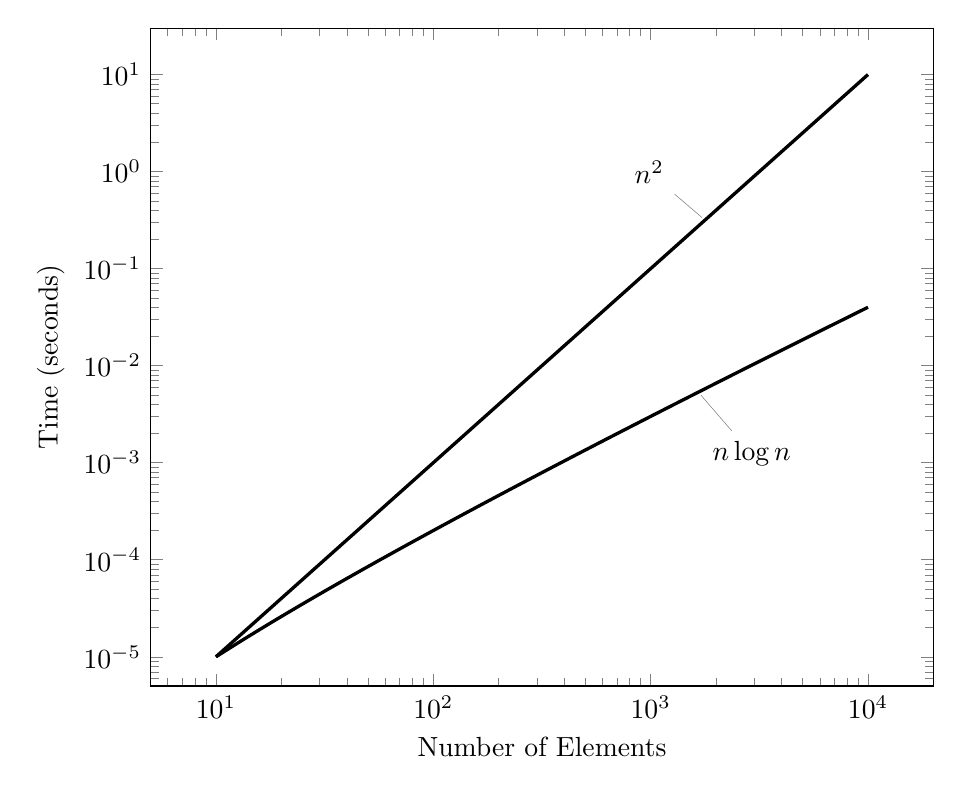
\begin{tikzpicture}
  \begin{loglogaxis}[ymode=log,
               xlabel={Number of Elements},
               ylabel={Time (seconds)},
               ymin=0.000005,
               ymax=30,
               width=.95\linewidth]
    \addplot[smooth, line width=1.2pt, domain=10:10000] {0.000001 * x * log10(x)} node[pos=0.75,pin={-85:$n \log{n}$},inner sep=0pt]{};
    \addplot[smooth, line width=1.2pt, domain=10:10000] {0.0000001 * x^2} node[pos=0.75,pin={140:$n^2$},inner sep=0pt]{};
  \end{loglogaxis}
\end{tikzpicture}\end{center}
\caption{Normalized Efficiency Approximations}
\end{figure}
\end{minipage}
\begin{minipage}{.5\linewidth}
\begin{figure}[H]
\begin{center}
\begin{tikzpicture}
  \begin{loglogaxis}[
               xlabel={Number of Elements},
               ylabel={Time (seconds)},
               ymin=0.000005,
               ymax=30,
               width=.95\linewidth]
    \addplot[smooth, color=red] file[]{01-graph-data/01-results-first-unsorted.data} node[pos=0.75,pin={-85:Unsorted},inner sep=0pt]{};
    \addplot[smooth, color=blue] file[]{01-graph-data/01-results-first-sorted.data} node[pos=0.75,pin={140:Sorted},inner sep=0pt]{};
  \end{loglogaxis}
\end{tikzpicture}
\end{center}
\caption{Left-most Pivot Selection}
\end{figure}
\end{minipage} \\[2em]

\begin{minipage}{.5\linewidth}
\begin{figure}[H]
\begin{center}
\begin{tikzpicture}
  \begin{loglogaxis}[
               xlabel={Number of Elements},
               ylabel={Time (seconds)},
               ymin=0.000005,
               ymax=30,
               width=.95\linewidth]
    \addplot[smooth, color=red] file[]{01-graph-data/01-results-last-unsorted.data} node[pos=0.75,pin={-85:Unsorted},inner sep=0pt]{};
    \addplot[smooth, color=blue] file[]{01-graph-data/01-results-last-sorted.data} node[pos=0.75,pin={140:Sorted},inner sep=0pt]{};
  \end{loglogaxis}
\end{tikzpicture}
\end{center}
\caption{Right-most Pivot Selection}
\end{figure}
\end{minipage}
\begin{minipage}{.5\linewidth}
\begin{figure}[H]
\begin{center}
\begin{tikzpicture}
  \begin{loglogaxis}[
               xlabel={Number of Elements},
               ylabel={Time (seconds)},
               ymin=0.000005,
               ymax=30,
               width=.95\linewidth]
    \addplot[smooth, color=red] file[]{01-graph-data/01-results-mid-unsorted.data} node[pos=0.75,pin={140:Unsorted},inner sep=0pt]{};
    \addplot[smooth, color=blue] file[]{01-graph-data/01-results-mid-sorted.data} node[pos=0.75,pin={-85:Sorted},inner sep=0pt]{};
  \end{loglogaxis}
\end{tikzpicture}\end{center}
\caption{Midpoint Pivot Selection}
\end{figure}
\end{minipage}

\begin{minipage}{.5\linewidth}
\begin{figure}[H]
\begin{center}
\begin{tikzpicture}
  \begin{loglogaxis}[
               xlabel={Number of Elements},
               ylabel={Time (seconds)},
               ymin=0.000005,
               ymax=30,
               width=.95\linewidth]
    \addplot[smooth, color=red] file[]{01-graph-data/01-results-random-unsorted.data} node[pos=0.75,pin={140:Unsorted},inner sep=0pt]{};
    \addplot[smooth, color=blue] file[]{01-graph-data/01-results-random-sorted.data} node[pos=0.75,pin={-85:Sorted},inner sep=0pt]{};
  \end{loglogaxis}
\end{tikzpicture}\end{center}
\caption{Random Pivot Selection}
\end{figure}
\end{minipage}
\begin{minipage}{.5\linewidth}
\begin{figure}[H]
\begin{center}
\begin{tikzpicture}
  \begin{loglogaxis}[
               xlabel={Number of Elements},
               ylabel={Time (seconds)},
               ymin=0.000005,
               ymax=30,
               width=.95\linewidth]
    \addplot[smooth, color=red] file[]{01-graph-data/01-results-med-unsorted.data} node[pos=0.75,pin={140:Unsorted},inner sep=0pt]{};
    \addplot[smooth, color=blue] file[]{01-graph-data/01-results-med-sorted.data} node[pos=0.75,pin={-85:Sorted},inner sep=0pt]{};
  \end{loglogaxis}
\end{tikzpicture}\end{center}
\caption{Median Pivot Selection}
\end{figure}
\end{minipage}

\begin{minipage}{.5\linewidth}
\begin{figure}[H]
\begin{center}
\begin{tikzpicture}
  \begin{loglogaxis}[ymode=log,
               xlabel={Number of Elements},
               ylabel={Time (seconds)},
               ymin=0.000005,
               ymax=30,
               width=.95\linewidth]
    \addplot[smooth, color=red] file[]{01-graph-data/01-results-first-unsorted.data} node[pos=0.42,pin={-85:First},inner sep=0pt]{};
    \addplot[smooth, color=blue] file[]{01-graph-data/01-results-last-unsorted.data} node[pos=0.58,pin={-85:Last},inner sep=0pt]{};
    \addplot[smooth, color=green] file[]{01-graph-data/01-results-mid-unsorted.data} node[pos=0.25,pin={-85:Midpoint},inner sep=0pt]{};
    \addplot[smooth, color=purple] file[]{01-graph-data/01-results-random-unsorted.data} node[pos=0.5,pin={140:Random},inner sep=0pt]{};
    \addplot[smooth, color=orange] file[]{01-graph-data/01-results-med-unsorted.data} node[pos=0.75,pin={-85:Median},inner sep=0pt]{};
  \end{loglogaxis}
\end{tikzpicture}\end{center}
\caption{All Pivot Selections on Unsorted Data}
\end{figure}
\end{minipage}
\begin{minipage}{.5\linewidth}
\begin{figure}[H]
\begin{center}
\begin{tikzpicture}
  \begin{loglogaxis}[ymode=log,
               xlabel={Number of Elements},
               ylabel={Time (seconds)},
               ymin=0.000005,
               ymax=30,
               width=.95\linewidth]
    \addplot[smooth, color=red] file[]{01-graph-data/01-results-first-sorted.data} node[pos=0.33,pin={150:First},inner sep=0pt]{};
    \addplot[smooth, color=blue] file[]{01-graph-data/01-results-last-sorted.data} node[pos=0.67,pin={150:Last},inner sep=0pt]{};
    \addplot[smooth, color=green] file[]{01-graph-data/01-results-mid-sorted.data} node[pos=0.25,pin={-85:Midpoint},inner sep=0pt]{};
    \addplot[smooth, color=purple] file[]{01-graph-data/01-results-random-sorted.data} node[pos=0.5,pin={-85:Random},inner sep=0pt]{};
    \addplot[smooth, color=orange] file[]{01-graph-data/01-results-med-sorted.data} node[pos=0.75,pin={-85:Median},inner sep=0pt]{};
  \end{loglogaxis}
\end{tikzpicture}\end{center}
\caption{All Pivot Selections on Sorted Data}
\end{figure}
\end{minipage}

\section*{Problem 2 [COMPLETE]}

\subsection*{Greedy 0-1 Knapsack}
\subsubsection*{Process}

In this case, the greedy function is maximized for price, packing the knapsack with items in descending order of price, until no more items can be added without exceeding the maximum capacity of the knapsack.

\begin{algorithm}[H]
\caption{Greedily pack a knapsack with items based on price}
\textbf{Inputs:} A given capacity (weight limit) $W$, and $S$, a set of items, each having a $weight$ and $price$. \\
\textbf{Outputs:} $L$, a subset of $S$, consisting of the items to be packed. $w$, the packed weight. $p$ the packed value. \\
\textbf{Complexity:} $O(n)$. Each item is computed against one time. \\[-0.8em]
\hline
\begin{algorithmic}[1]
  \State \Call{SortDescending}{$S$, $price$} \Comment{Sort the items by price, descending}
  \State $w \leftarrow 0$ \Comment{Weight accumulator}
  \State $p \leftarrow 0$ \Comment{Price accumulator}
  \State $L \leftarrow \{\}$
  \ForAll{$s$ \textbf{in} $S$} 
    \If {$w + s.weight \leq W$} \Comment{Item can fit}
      \State $w \leftarrow w + s.weight$ \Comment{Accumulate the weight}
      \State $p \leftarrow p + s.price$ \Comment{Accumulate the price}
      \State $L \leftarrow L\cup\{s\}$ \Comment{Merge the item into the output set}
    \EndIf
  \EndFor
\end{algorithmic}
\end{algorithm}

\subsubsection*{Solution}

Given weights of $\left\{ 20, 24, 14, 20, 18, 20, 10, 6 \right\}$, prices of $\left\{ 15, 9, 27, 12, 36, 12, 9, 12 \right\}$, and a maximum capacity of $80$, the optimal 0-1 solution is:

\begin{table}[H]
\begin{center}
\begin{tabular}{rr||rr}
\multicolumn{2}{c||}{Item} & \multicolumn{2}{c}{Total} \\
\multicolumn{1}{c}{Weight} & \multicolumn{1}{c||}{Price} & \multicolumn{1}{c}{Weight} & \multicolumn{1}{c}{Price} \\
\hline
18 & 36 & 18 &  36 \\
14 & 27 & 32 &  63 \\
20 & 15 & 52 &  78 \\
20 & 12 & 72 &  90 \\
 6 & 12 & \textbf{78} & \textbf{102} \\
\end{tabular}
\end{center}
\caption{Greedy 0-1 Knapsack Solution}
\end{table}

\pagebreak
\subsection*{Greedy Fractional Knapsack}
\subsubsection*{Process}

In this case, the greedy function is maximized for value ($weight \div price$), packing the knapsack with items in descending order of value, until no more items can be added without exceeding the maximum capacity of the knapsack. At this point, the fraction of the next item is calculated and added to the knapsack, thereby reaching the maximum capacity while ensuring the maximum possible value.

\begin{algorithm}[H]
\caption{Greedily pack a knapsack with items based on value, including a fractional quantity}
\textbf{Inputs:} A given capacity (weight limit) $W$, and $S$, a set of items, each having a $weight$, $price$, and $quantity$ (default/maximum 1.0). \\
\textbf{Outputs:} $L$, a subset of $S$, consisting of the items to be packed. $w$, the packed weight. $p$ the packed value. \\
\textbf{Complexity:} $O(n)$. Each item is computed against one time. \\[-0.8em]
\hline
\begin{algorithmic}[1]
  \State \Call{SortDescending}{$S$, $price$} \Comment{Sort the items by price, descending}
  \State $w \leftarrow 0$ \Comment{Weight accumulator}
  \State $p \leftarrow 0$ \Comment{Price accumulator}
  \State $L \leftarrow \{\}$
  \ForAll{$s$ \textbf{in} $S$} 
    \If {$w + s.weight \leq W$} \Comment{Item can fit}
      \State $w \leftarrow w + s.weight$ \Comment{Accumulate the weight}
      \State $p \leftarrow p + s.price$ \Comment{Accumulate the price}
      \State $L \leftarrow L\cup\{s\}$ \Comment{Merge the item into the output set}
    \Else
      \State $s.quantity \leftarrow \frac{W - w}{s.weight}$ \Comment{Adjust the quantity}
      \State $w \leftarrow w + (s.weight * s.quantity)$ \Comment{Accumulate the modified weight}
      \State $p \leftarrow p + s.price * s.quantity)$ \Comment{Accumulate the modified price}
      \State $L \leftarrow L\cup\{s\}$ \Comment{Merge the item into the output set}
    \EndIf
  \EndFor
\end{algorithmic}
\end{algorithm}

\subsubsection*{Solution}

Given weights of $\left\{ 20, 24, 14, 20, 18, 20, 10, 6 \right\}$, prices of $\left\{ 15, 9, 27, 12, 36, 12, 9, 12 \right\}$, and a maximum capacity of $80$, the optimal fractional solution is:

\begin{table}[H]
\begin{center}
\begin{tabular}{rrrr||rr}
\multicolumn{4}{c||}{Item} & \multicolumn{2}{c}{Total} \\
\multicolumn{1}{c}{Weight} & \multicolumn{1}{c}{Price} & \multicolumn{1}{c}{Value} & \multicolumn{1}{c||}{Quantity} & \multicolumn{1}{c}{Weight} & \multicolumn{1}{c}{Price} \\
\hline
18 & 36 & 2.00 & 1.0 & 18 &  36 \\
 6 & 12 & 2.00 & 1.0 & 24 &  48 \\
14 & 27 & 1.93 & 1.0 & 32 &  63 \\
10 &  9 & 0.90 & 1.0 & 52 &  78 \\
20 & 15 & 0.75 & 1.0 & 72 &  90 \\
20 & 12 & 0.60 & 0.6 & \textbf{80} & \textbf{106.2} \\
\end{tabular}
\end{center}
\caption{Greedy Fractional Knapsack Solution}
\end{table}

\section*{Problem 3 [COMPLETE]}

\begin{figure}[H]
\begin{center}
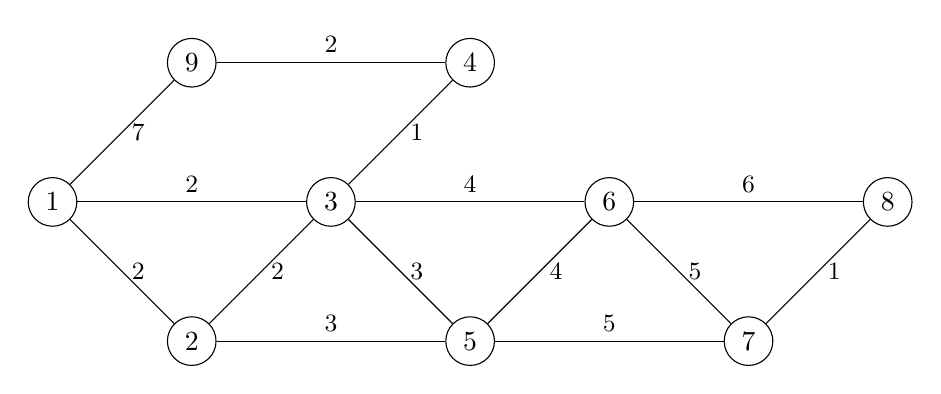
\begin{tikzpicture}[auto,node distance=2.5cm,main node/.style={circle,draw}]

  \node[main node] (1) {1};
  \node[main node] (2) [below right of=1] {2};
  \node[main node] (3) [above right of=2] {3};
  \node[main node] (4) [above right of=3] {4};
  \node[main node] (5) [below right of=3] {5};
  \node[main node] (6) [below right of=4] {6};
  \node[main node] (7) [below right of=6] {7};
  \node[main node] (8) [above right of=7] {8};
  \node[main node] (9) [above right of=1] {9};
  
  \path[every node/.style={font=\small}]
    (1) edge node [right] {2} (2)
    (2) edge node [right] {2} (3)
    (1) edge node [above] {2} (3)
    (1) edge node [right] {7} (9)
    (9) edge node [above] {2} (4)
    (3) edge node [right] {1} (4)
    (2) edge node [above] {3} (5)
    (5) edge node [right] {3} (3)
    (3) edge node [above] {4} (6)
    (5) edge node [right] {4} (6)
    (5) edge node [above] {5} (7)
    (6) edge node [right] {5} (7)
    (6) edge node [above] {6} (8)
    (7) edge node [right] {1} (8);
\end{tikzpicture}
\end{center}
\caption{Undirected Graph}
\end{figure}

\subsection*{Minimum Spanning Tree}

To create the minimum spanning tree (MST), iterate through the edges (in order of weight -- Kruskal's Algorithm), taking into consideration only edges with the weight of the current wave (e.g., 1, 2, 3, \ldots). The edge is a member of the MST if and only if the edge can be added to the MST without creating a cycle (a closed area within the graph). \\

\begin{enumerate}
 \item[Wave 1]
\begin{center}
\adjustbox{valign=t}{
\begin{tikzpicture}[auto,node distance=2.5cm,main node/.style={circle,draw}]
  \node[main node] (1) {1};
  \node[main node] (2) [below right of=1] {2};
  \node[main node] (3) [above right of=2] {3};
  \node[main node] (4) [above right of=3] {4};
  \node[main node] (5) [below right of=3] {5};
  \node[main node] (6) [below right of=4] {6};
  \node[main node] (7) [below right of=6] {7};
  \node[main node] (8) [above right of=7] {8};
  \node[main node] (9) [above right of=1] {9};
  
  \path[line width=1.2pt, every node/.style={font=\small}]
    (3) edge node [right] {1} (4)
    (7) edge node [right] {1} (8);
\end{tikzpicture} 
} \\[3em]
\end{center} 

 \item[Wave 2]
\begin{center}
\adjustbox{valign=t}{
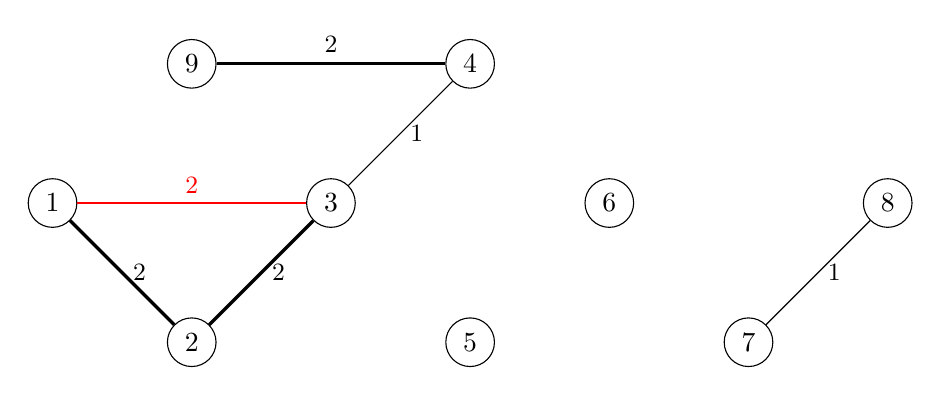
\begin{tikzpicture}[auto,node distance=2.5cm,main node/.style={circle,draw}]
  \node[main node] (1) {1};
  \node[main node] (2) [below right of=1] {2};
  \node[main node] (3) [above right of=2] {3};
  \node[main node] (4) [above right of=3] {4};
  \node[main node] (5) [below right of=3] {5};
  \node[main node] (6) [below right of=4] {6};
  \node[main node] (7) [below right of=6] {7};
  \node[main node] (8) [above right of=7] {8};
  \node[main node] (9) [above right of=1] {9};
  
  \path[every node/.style={font=\small}]
    (3) edge node [right] {1} (4)
    (7) edge node [right] {1} (8);
    
  \path[line width=1.2pt, every node/.style={font=\small}]
    (1) edge node [right] {2} (2)
    (2) edge node [right] {2} (3)
    (9) edge node [above] {2} (4);
    
  \path[color=red, every node/.style={font=\small, color=red}]
    (1) edge node [above] {2} (3);
\end{tikzpicture}
} \\[3em]
\end{center}

\item[Wave 3]
\begin{center}
\adjustbox{valign=t}{
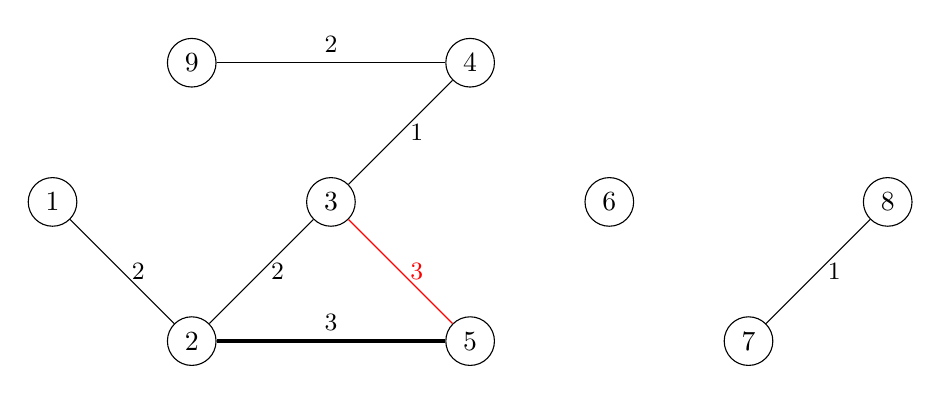
\begin{tikzpicture}[auto,node distance=2.5cm,main node/.style={circle,draw}]
  \node[main node] (1) {1};
  \node[main node] (2) [below right of=1] {2};
  \node[main node] (3) [above right of=2] {3};
  \node[main node] (4) [above right of=3] {4};
  \node[main node] (5) [below right of=3] {5};
  \node[main node] (6) [below right of=4] {6};
  \node[main node] (7) [below right of=6] {7};
  \node[main node] (8) [above right of=7] {8};
  \node[main node] (9) [above right of=1] {9};
  
  \path[every node/.style={font=\small}]
    (3) edge node [right] {1} (4)
    (7) edge node [right] {1} (8)
    (1) edge node [right] {2} (2)
    (2) edge node [right] {2} (3)
    (9) edge node [above] {2} (4);
    
  \path[line width=1.2pt, every node/.style={font=\small}]
    (2) edge node [above] {3} (5);
    
  \path[color=red, every node/.style={font=\small, color=red}]
    (5) edge node [right] {3} (3);
\end{tikzpicture}
} \\[3em]
\end{center}

\item[Wave 4]
\begin{center}
\adjustbox{valign=t}{
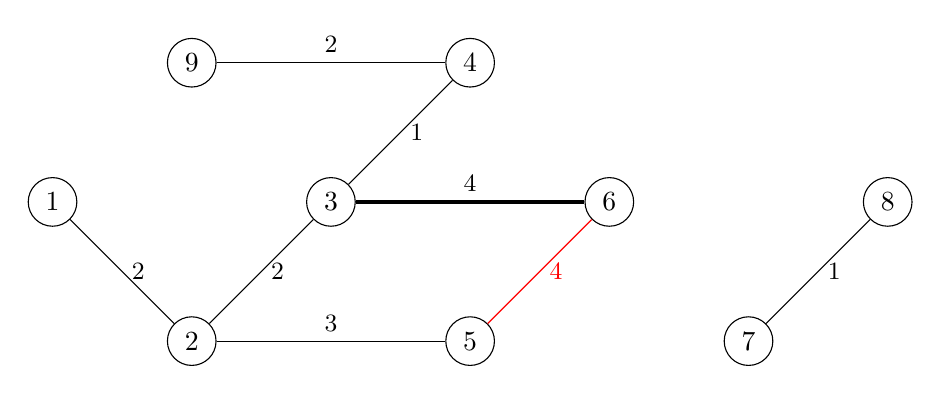
\begin{tikzpicture}[auto,node distance=2.5cm,main node/.style={circle,draw}]
  \node[main node] (1) {1};
  \node[main node] (2) [below right of=1] {2};
  \node[main node] (3) [above right of=2] {3};
  \node[main node] (4) [above right of=3] {4};
  \node[main node] (5) [below right of=3] {5};
  \node[main node] (6) [below right of=4] {6};
  \node[main node] (7) [below right of=6] {7};
  \node[main node] (8) [above right of=7] {8};
  \node[main node] (9) [above right of=1] {9};
  
  \path[every node/.style={font=\small}]
    (3) edge node [right] {1} (4)
    (7) edge node [right] {1} (8)
    (1) edge node [right] {2} (2)
    (2) edge node [right] {2} (3)
    (9) edge node [above] {2} (4)
    (2) edge node [above] {3} (5);
    
  \path[line width=1.2pt, every node/.style={font=\small}]
    (3) edge node [above] {4} (6);
    
  \path[color=red, every node/.style={font=\small, color=red}]
    (5) edge node [right] {4} (6);
\end{tikzpicture}
} \\[3em]
\end{center}

\item[Wave 5]
\begin{center}
\adjustbox{valign=t}{
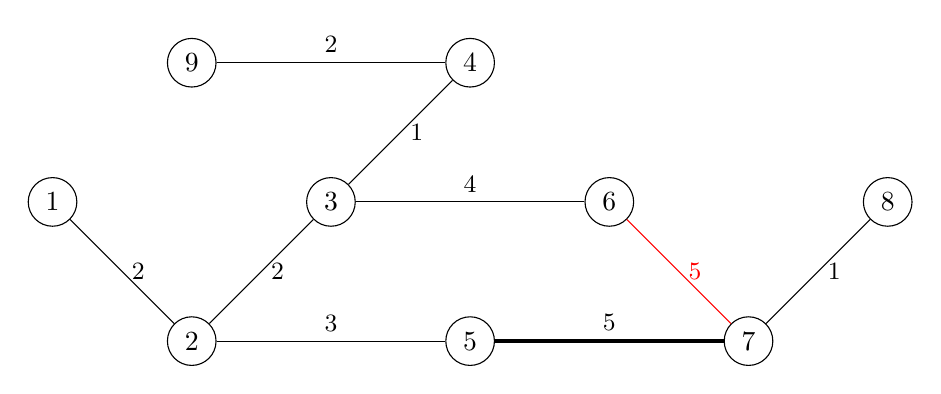
\begin{tikzpicture}[auto,node distance=2.5cm,main node/.style={circle,draw}]
  \node[main node] (1) {1};
  \node[main node] (2) [below right of=1] {2};
  \node[main node] (3) [above right of=2] {3};
  \node[main node] (4) [above right of=3] {4};
  \node[main node] (5) [below right of=3] {5};
  \node[main node] (6) [below right of=4] {6};
  \node[main node] (7) [below right of=6] {7};
  \node[main node] (8) [above right of=7] {8};
  \node[main node] (9) [above right of=1] {9};
  
  \path[every node/.style={font=\small}]
    (3) edge node [right] {1} (4)
    (7) edge node [right] {1} (8)
    (1) edge node [right] {2} (2)
    (2) edge node [right] {2} (3)
    (9) edge node [above] {2} (4)
    (2) edge node [above] {3} (5)
    (3) edge node [above] {4} (6);
    
  \path[line width=1.2pt, every node/.style={font=\small}]
    (5) edge node [above] {5} (7);
    
  \path[color=red, every node/.style={font=\small, color=red}]
    (6) edge node [right] {5} (7);
\end{tikzpicture}
} \\[3em]
\end{center}

\item[Wave 6]
\begin{center}
\adjustbox{valign=t}{
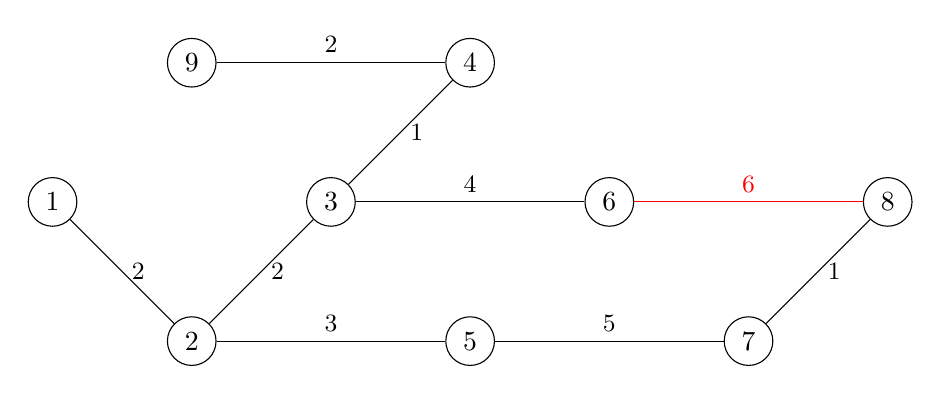
\begin{tikzpicture}[auto,node distance=2.5cm,main node/.style={circle,draw}]
  \node[main node] (1) {1};
  \node[main node] (2) [below right of=1] {2};
  \node[main node] (3) [above right of=2] {3};
  \node[main node] (4) [above right of=3] {4};
  \node[main node] (5) [below right of=3] {5};
  \node[main node] (6) [below right of=4] {6};
  \node[main node] (7) [below right of=6] {7};
  \node[main node] (8) [above right of=7] {8};
  \node[main node] (9) [above right of=1] {9};
  
  \path[every node/.style={font=\small}]
    (3) edge node [right] {1} (4)
    (7) edge node [right] {1} (8)
    (1) edge node [right] {2} (2)
    (2) edge node [right] {2} (3)
    (9) edge node [above] {2} (4)
    (2) edge node [above] {3} (5)
    (3) edge node [above] {4} (6)
    (5) edge node [above] {5} (7);
    
  \path[color=red, every node/.style={font=\small, color=red}]
    (6) edge node [above] {6} (8);
\end{tikzpicture}
} \\[3em]
\end{center}

\item[Wave 7]
\begin{center}
\adjustbox{valign=t}{
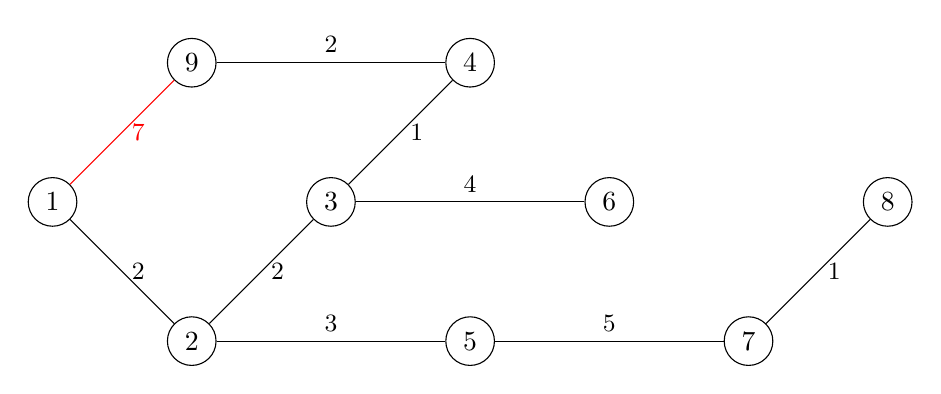
\begin{tikzpicture}[auto,node distance=2.5cm,main node/.style={circle,draw}]
  \node[main node] (1) {1};
  \node[main node] (2) [below right of=1] {2};
  \node[main node] (3) [above right of=2] {3};
  \node[main node] (4) [above right of=3] {4};
  \node[main node] (5) [below right of=3] {5};
  \node[main node] (6) [below right of=4] {6};
  \node[main node] (7) [below right of=6] {7};
  \node[main node] (8) [above right of=7] {8};
  \node[main node] (9) [above right of=1] {9};
  
  \path[every node/.style={font=\small}]
    (3) edge node [right] {1} (4)
    (7) edge node [right] {1} (8)
    (1) edge node [right] {2} (2)
    (2) edge node [right] {2} (3)
    (9) edge node [above] {2} (4)
    (2) edge node [above] {3} (5)
    (3) edge node [above] {4} (6)
    (5) edge node [above] {5} (7);
    
  \path[color=red, every node/.style={font=\small, color=red}]
    (1) edge node [right] {7} (9);
\end{tikzpicture}
} \\[3em]
\end{center}

\item[Final]
\begin{figure}[H]
\begin{center}
\adjustbox{valign=t}{
\begin{tikzpicture}[auto,node distance=2.5cm,main node/.style={circle,draw}]
  \node[main node] (1) {1};
  \node[main node] (2) [below right of=1] {2};
  \node[main node] (3) [above right of=2] {3};
  \node[main node] (4) [above right of=3] {4};
  \node[main node] (5) [below right of=3] {5};
  \node[main node] (6) [below right of=4] {6};
  \node[main node] (7) [below right of=6] {7};
  \node[main node] (8) [above right of=7] {8};
  \node[main node] (9) [above right of=1] {9};
  
  \path[every node/.style={font=\small}]
    (3) edge node [right] {1} (4)
    (7) edge node [right] {1} (8)
    (1) edge node [right] {2} (2)
    (2) edge node [right] {2} (3)
    (9) edge node [above] {2} (4)
    (2) edge node [above] {3} (5)
    (3) edge node [above] {4} (6)
    (5) edge node [above] {5} (7);
\end{tikzpicture}
} \\[10pt]
\end{center}
\caption{Minimum Spanning Tree}
\end{figure}

\end{enumerate}

\subsection*{Greedy Single Source Shortest Path}

\subsubsection*{Process}

The answer to this problem can be derived using Dijkstra's algorithm. In the following table, $u$ refers to the node of context for each iteration of the loop, while all other values represent the distance from node 1.

\begin{table}[H]
\begin{center}
\begin{tabular}{c|ccccccccc}
$u$ & 
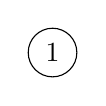
\begin{tikzpicture}[auto,node distance=2.5cm,main node/.style={circle,draw}] \node[main node] (1) {1}; \end{tikzpicture} & 
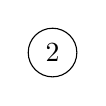
\begin{tikzpicture}[auto,node distance=2.5cm,main node/.style={circle,draw}] \node[main node] (2) {2}; \end{tikzpicture} & 
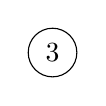
\begin{tikzpicture}[auto,node distance=2.5cm,main node/.style={circle,draw}] \node[main node] (3) {3}; \end{tikzpicture} & 
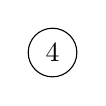
\begin{tikzpicture}[auto,node distance=2.5cm,main node/.style={circle,draw}] \node[main node] (4) {4}; \end{tikzpicture} & 
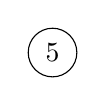
\begin{tikzpicture}[auto,node distance=2.5cm,main node/.style={circle,draw}] \node[main node] (5) {5}; \end{tikzpicture} & 
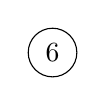
\begin{tikzpicture}[auto,node distance=2.5cm,main node/.style={circle,draw}] \node[main node] (6) {6}; \end{tikzpicture} & 
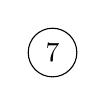
\begin{tikzpicture}[auto,node distance=2.5cm,main node/.style={circle,draw}] \node[main node] (7) {7}; \end{tikzpicture} & 

\begin{tikzpicture}[auto,node distance=2.5cm,main node/.style={circle,draw}] \node[main node] (8) {8}; \end{tikzpicture} & 
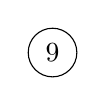
\begin{tikzpicture}[auto,node distance=2.5cm,main node/.style={circle,draw}] \node[main node] (9) {9}; \end{tikzpicture} \\
\hline \\[-0.97em]
  & 0 &  $\infty$  &  $\infty$  &  $\infty$  &  $\infty$  &  $\infty$  &   $\infty$  &   $\infty$  &  $\infty$  \\
\hline \\[-0.9em]
1 & 0 & \textbf{2} & \textbf{2} &  $\infty$  &  $\infty$  &  $\infty$  &   $\infty$  &   $\infty$  & \textbf{7} \\
2 & 0 &         2  &         2  &  $\infty$  & \textbf{5} &  $\infty$  &   $\infty$  &   $\infty$  &         7  \\
3 & 0 &         2  &         2  & \textbf{3} &         5  & \textbf{6} &   $\infty$  &   $\infty$  &         7  \\
4 & 0 &         2  &         2  &         3  &         5  &         6  &   $\infty$  &   $\infty$  & \textbf{5} \\
5 & 0 &         2  &         2  &         3  &         5  &         6  & \textbf{10} &   $\infty$  &         5  \\
9 & 0 &         2  &         2  &         3  &         5  &         6  &         10  &   $\infty$  &         5  \\
6 & 0 &         2  &         2  &         3  &         5  &         6  &         10  & \textbf{12} &         5  \\
7 & 0 &         2  &         2  &         3  &         5  &         6  &         10  & \textbf{11} &         5  \\
8 & 0 &         2  &         2  &         3  &         5  &         6  &         10  &         11  &         5  \\
\end{tabular}
\end{center}
\caption{Distance Trace of Dijkstra's Single Source Shortest Path Algorithm}
\end{table}

\subsubsection*{Solution}

\begin{figure}[H]
\begin{center}
\adjustbox{valign=t}{
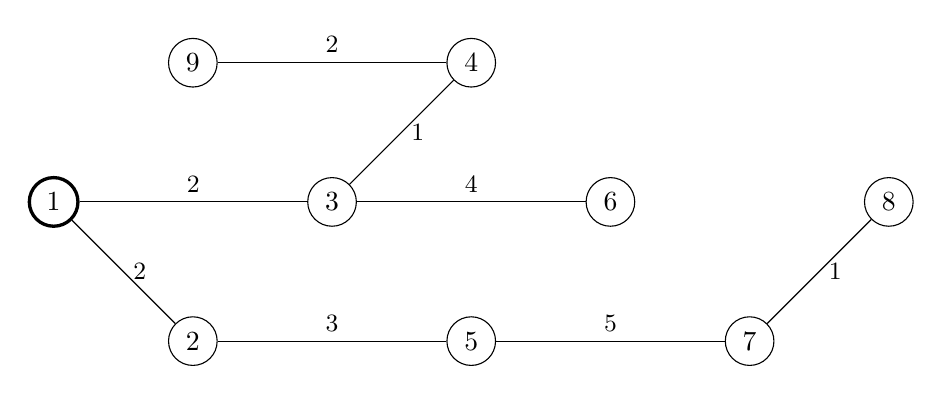
\begin{tikzpicture}[auto,node distance=2.5cm,main node/.style={circle,draw}]
  \node[main node, line width=1.2pt] (1) {1};
  \node[main node] (2) [below right of=1] {2};
  \node[main node] (3) [above right of=2] {3};
  \node[main node] (4) [above right of=3] {4};
  \node[main node] (5) [below right of=3] {5};
  \node[main node] (6) [below right of=4] {6};
  \node[main node] (7) [below right of=6] {7};
  \node[main node] (8) [above right of=7] {8};
  \node[main node] (9) [above right of=1] {9};
  
  \path[every node/.style={font=\small}]
    (3) edge node [right] {1} (4)
    (7) edge node [right] {1} (8)
    (1) edge node [right] {2} (2)
    (1) edge node [above] {2} (3)
    (9) edge node [above] {2} (4)
    (2) edge node [above] {3} (5)
    (3) edge node [above] {4} (6)
    (5) edge node [above] {5} (7);
\end{tikzpicture}
} \\[10pt]
\end{center}
\caption{Dijkstra's Single Source Shortest Path Tree}
\end{figure}

\section*{Problem 4 [COMPLETE]}

\subsection*{Process}
\begin{algorithm}[H]
\caption{Greedily schedule a number of lecture halls for a set of activities}
\textbf{Inputs:} $S$, a set of activities, where each element $s$ has a $start$ and $finish$ property, and $s.start < s.finish$. \\
\textbf{Outputs:} L, a set of non-conflicting schedule sets. \\
\textbf{Complexity:} $O(n\log{n})$. Each node is computed against one time, without replacement.
\hline
\begin{algorithmic}[1]
    \State Sort S descending by $finish$
    \State $L = \left\{\right\}$
    \State $i = 0$
    \While {$S$ has elements}
      \State $j = 1$
      \ForAll {$s$ \textbf{in} $S$} 
            \If {$s_{start} \geq j$}
                 \State $L_i = L_i\cup\left\{s\right\}$
                 \State $j = s_{finish}$
                 \State Remove $s$ from $S$
            \EndIf
      \EndFor
      \State $i = i + 1$
    \EndWhile
\end{algorithmic}
\end{algorithm}

\subsection*{Solution}

%Lecture Hall
%  1 -> 3
%  4 -> 5
%  6 -> 7
%Lecture Hall
%  2 -> 5
%Lecture Hall
%  4 -> 7

\begin{figure}[H]
\begin{center}
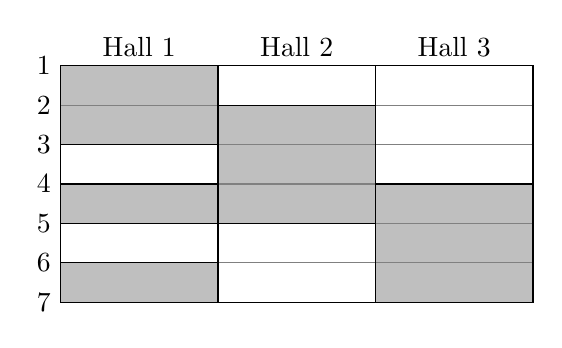
\begin{tikzpicture}
    \draw [white] (1,0) -- (1,3) node [text=black,above] {Hall 1}
                  (3,0) -- (3,3) node [text=black,above] {Hall 2}
                  (5,0) -- (5,3) node [text=black,above] {Hall 3};

    \draw [gray] (6,3.0) -- (0,3.0) node [text=black,left] {1}
                 (6,2.5) -- (0,2.5) node [text=black,left] {2}
                 (6,2.0) -- (0,2.0) node [text=black,left] {3}
                 (6,1.5) -- (0,1.5) node [text=black,left] {4}
                 (6,1.0) -- (0,1.0) node [text=black,left] {5}
                 (6,0.5) -- (0,0.5) node [text=black,left] {6}
                 (6,0.0) -- (0,0.0) node [text=black,left] {7};
    
    \draw [fill=none] (0,0) rectangle (2,3)
                      (2,0) rectangle (4,3)
                      (4,0) rectangle (6,3);

    \draw [fill=gray,fill opacity=0.5] (0,3.0) rectangle (2,2)
                                       (0,1.5) rectangle (2,1)
                                       (0,0.5) rectangle (2,0)
                                       (2,2.5) rectangle (4,1)
                                       (4,1.5) rectangle (6,0);
                      
\end{tikzpicture}
\end{center}
\caption{Scheduling Problem Solution}
\end{figure}

\section*{Problem 5 [COMPLETE]}

Although both Prim and Kruskal's algorithms are defined using graphs that have positive edge weights, both will correctly function given input edged that have negative weights. Both algorithms iterate through the graph, visiting and declaring edges "safe" if they do not create a cycle in the graph (an enclosed area). Thus, both algorithms will create a MST regardless of input edge weight.

\end{document}
